\documentclass[12pt,a4paper]{article}
\usepackage[utf8]{inputenc}
\usepackage[T1]{fontenc} 
\usepackage[french]{babel}
\usepackage{fullpage}
\usepackage{amsmath}
\usepackage{amsfonts}
\usepackage{amssymb}
\usepackage{color}
\usepackage{titlesec}
\usepackage[french]{varioref}
\usepackage{graphicx}
\usepackage{subfig}
\usepackage{indentfirst}
\usepackage{tocloft}
\usepackage[backend=bibtex,bibstyle=authoryear]{biblatex}
\usepackage{url}
\usepackage{natbib}

% Aerer les tableaux
\renewcommand{\arraystretch}{1.5}
\setlength{\tabcolsep}{0.5cm}

\makeatletter
\definecolor{vert}{rgb}{0,0.5,0}
\definecolor{vertclair}{rgb}{0.85,1,0.85}
\definecolor{redclair}{rgb}{1,0.9,0.75}

\titleformat*{\section}{\color{red}\scshape\bfseries\LARGE}
\titleformat*{\subsection}{\scshape\bfseries\large}
\titleformat*{\subsubsection}{\normalsize\bfseries}

\titlespacing*{\section}{0cm}{0.5cm}{0.5cm}
\titlespacing*{\subsection}{1cm}{0.5cm}{0.3cm}
\titlespacing*{\subsubsection}{1.75cm}{0.3cm}{0.3cm}

\renewcommand{\thesection}{\textcolor{red}{\Roman{section}}}
\renewcommand{\thesubsection}{\textcolor{blue}{\Alph{subsection}}}
\renewcommand{\thesubsubsection}{\textcolor{vert}{\arabic{subsubsection}}}

\newcommand{\mnp}[1]{\mathcal{M}_{n,p}\left(\bb{#1}\right)}

% Le vocabulaire
\newcommand{\vocabulaire}[1]{\\ \begin{minipage}{1\textwidth}\textbf{Vocabulaire :} \begin{center}\begin{minipage}{0.8\textwidth}
        #1
      \end{minipage}\end{center}\end{minipage}}

% les théorèmes
\newtheorem{thm}{\textsc{Théorème}}
\newcommand{\theoreme}[2]{
  \begin{center}
    \fcolorbox{red}{redclair}{
      \begin{minipage}{0.9\textwidth}
        \begin{thm}[\emph{#1}] \color{red} \ \newline
              #2
        \end{thm}
      \end{minipage}}
  \end{center}}

% Résultat important
\newcommand{\important}[1]{
  \vskip 0.5cm
  \fcolorbox{red}{white}{
    \begin{minipage}[c]{0.9\linewidth}
      #1
    \end{minipage}
  }
  \vskip 0.5cm
}

% Les remarques
\newtheorem{rmq}{Remarque}
\newcommand{\remarque}[1]{
  \fcolorbox{black}{white}{
    \begin{minipage}{1\textwidth}
      \begin{rmq}
        #1
      \end{rmq}
    \end{minipage}}\smallskip}

% Les lemmes
\newtheorem{lem}{\textsc{Lemme}}
\newcommand{\lemme}[2]{
  \begin{center}
    \fcolorbox{red}{white}{
      \begin{minipage}{0.9\textwidth}
        \begin{lem}
          \label{#1}
          \textcolor{red}{#2}
        \end{lem}
      \end{minipage}}
  \end{center}\smallskip}

% Les preuves
\newcounter{pr}
\newcommand{\preuve}[3]{
  \addtocounter{pr}{1}
  \begin{center}
    \begin{minipage}{0.6\textwidth}
      \begin{center}
        \textbf{Démonstration \thepr \enspace-- #2 \ref{#1}}
      \end{center}
      #3
    \end{minipage}
  \end{center}\smallskip}

% cas 1,2...
\newlength{\caslength}
\newcommand{\cas}[2]{
  \begin{flushright}
    \begin{minipage}{0.9\textwidth}
      \settowidth{\caslength}{Cas #1 : }
      \parbox[b]{\caslength}{\textbf{Cas #1 :}}
      \parbox[t]{0.8\textwidth}{#2}
    \end{minipage}
  \end{flushright}
}

% méthode
\newsavebox{\methodebox}
\newenvironment{methode}[1]
{\small\savebox{\methodebox}{\textsc{Méthode : #1 }}\usebox{\methodebox}\\
  \begin{tabular}{rl}}
  {\normalsize\end{tabular}}

\newtheorem{exempletheoreme}{\textbf{Exemple}}
\newenvironment{exemple}{
  \begin{exempletheoreme}\normalfont \
    \begin{center}
      \begin{minipage}{0.9\textwidth}}
      {\end{minipage}
    \end{center}
  \end{exempletheoreme}
}


% les définitions
\newtheorem{definitiontheoreme}{\textbf{Définition}}
\newcommand{\definition}[2]{
  \begin{center}
    \fcolorbox{vert}{vertclair}{
      \begin{minipage}{1\textwidth}
        \begin{definitiontheoreme} \normalfont (\emph{#1}) \color{vert} \newline
          #2
        \end{definitiontheoreme}
      \end{minipage}}
  \end{center}}

\usepackage{minted}
\usepackage{verbatim}
\let\verbatiminput=\verbatimtabinput
\everymath{\displaystyle}
\addtolength{\textheight}{1cm}

\makeindex
\begin{document}
\thispagestyle{empty}
\begin{minipage}{1\textwidth}
  \centering 

  \begin{flushleft}
    
\includegraphics[scale=0.3]{LogoSup.jpg}
    \newline

    \textbf{Supélec - Campus de Metz\\
      $2^{eme}$ année - Année 2013-2014}\\
    \textsc{Mars-Juin 2014}
  \end{flushleft}
  
  \vskip 5cm
  {\LARGE\textsc Projet de conception}
  \vskip 0.5cm
  {\LARGE\textsc Exploration d'Hadoop}
  \vskip 5cm

  \Large{Alexandre Careil \\
    Juan Manuel Mu\~noz Pérez}
\end{minipage}

%%% Local Variables: 
%%% mode: latex
%%% TeX-master: "CompteRendu"
%%% End: 

\thispagestyle{empty}
\newpage
\null
\thispagestyle{empty}
\newpage 

\tableofcontents
\thispagestyle{empty}
\newpage

\thispagestyle{empty}
\null
\newpage

% Introduction
\section{Introduction}

\par à compléter

%%% Local Variables: 
%%% mode: latex
%%% TeX-master: "CompteRendu"
%%% End: 


% Description du système de fichiers Hadoop (HDFS)
\section{Hadoop Distritubted File System}

\par HDFS pour \textit{Hadoop Distributed File System} est le système de fichiers propre à Hadoop. C'est le composant en charge du stockage des données dans un cluster Hadoop.

\par Alex je te laisse le soin de détailler HDFS...

\subsection{Fonctionnement}

\par Le fonctionnement de HDFS s'appuie sur plusieurs démons :

\begin{itemize}
\item le NameNode (NN) : c'est le noeud maître disposant d'une machine dédiée;
\item le SecondaryNameNode (SNN) : tout comme le NN c'est aussi un noeud maître disposant d'une machine dédiée. Ce noeud vient comme son nom l'indique seconder le NN en cas de panne majeure afin de ne pas perdre l'arborescense des données stockées dans le HDFS;
\item le DataNode (DN) : c'est un noeud esclave contenant les données du HDFS et implanté sur chaque machine du cluster.
\end{itemize}

\par A titre d'exemple, dans un cluster de 50 machines, vous trouverez trois noeuds maîtres correspondant au NameNode, SecondaryNameNode et JobTracker (confère partie suivante sur MapReduce). Il ne reste plus que 47 noeuds esclaves contenant chacun une copie du DataNode et du TaskTracker (confère partie suivante sur MapReduce). Détaillons les noeuds maîtres.

\subsubsection{Le NameNode}

\par à compléter

\subsubsection{Le SecondaryNameNode}

\par à compléter

%%% Local Variables: 
%%% mode: latex
%%% TeX-master: "CompteRendu"
%%% End: 


% Description du patron de conception MapReduce
\section{MapReduce}
\subsection{Présentation et fonctionnement}

\par MapReduce est un patron d'architecture de développement informatique, inventé par Google. Un de ses principaux objectifs est de réaliser des calculs parallèles et souvent distribués sur des jeux de données très volumineuses (de l'ordre du téraoctet, voire du pétaoctet). Compte tenu la volumétrie des données mises en jeu, il devient inconcevable de réaliser des traitements au cas par cas. La particularité de MapReduce réside en ce que le développeur Hadoop prend en considération qu'un seul enregistrement. La généralisation à l'ensemble des données est gérée par Hadoop.

\par Le fonctionnement de MapReduce se décompose en trois parties :
\begin{itemize}
\item le \textit{driver} s'exécutant chargé de configurer le job et de le soumettre pour exécution;
\item le \texttt{mapper} chargé de lire les données dans le HDFS et de les traiter;
\item le \texttt{reducer} chargé de consolider les résultats issus du \texttt{mapper} et de les écrire sur le HDFS. L'utilisateur peut ensuite les récupérer sur son disque local.
\end{itemize}

\par De manière très schématique, un programme MapReduce comporte toujours deux fonctions : \textit{map} et \textit{reduce} (cf. figure~\ref{fig:mapreduce-exp}). La première a pour tâche de parser les données présentes en entrée en un ensemble de paires \texttt{<clé, valeur>} envoyées en entrée de la fonction \textit{reduce} où \texttt{clé} et \texttt{valeur} sont entièrement définies par le développeur en fonction des besoins. Cette dernière se charge de la réduction des paires selon la \texttt{clé}. Il est essentiel d'avoir à l'esprit la spécialisation des n\oe{}uds esclaves en noeuds exécutant des fonctions \textit{map} ou des fonctions \textit{reduce} uniquement.

\begin{figure}[h!]
  \centering
  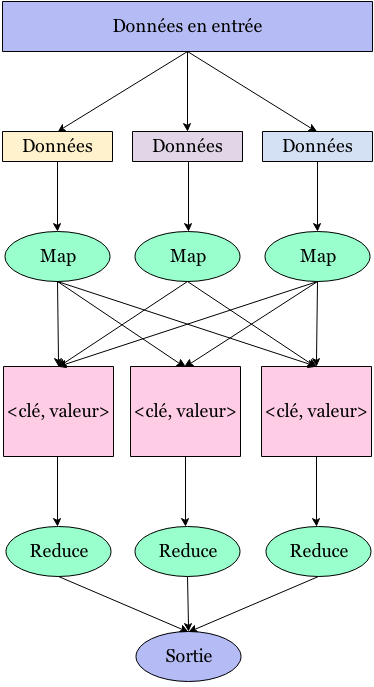
\includegraphics[scale=0.4]{images/mapreduce_arch.png}
  \caption{Architecture du patron MapReduce}
  \label{fig:mapreduce-exp}
\end{figure}

\par L'architecture Hadoop est développée dans le but de traiter une volumétrie de données très conséquente. Or il est clair qu'un facteur de ralentissement de traitement réside dans la transmission des données (lecture/écriture). Par conséquent, Hadoop esquive au plus cette limitation technologique en envoyant le code MapReduce dans les DataNodes où les données ont au préalable été transférées. Ce ne sont plus les données mais le code qui transite désormais, et ce à quelque exception près que nous détaillons ci-dessous.

\subsection{Shuffle \& Sort}

\paragraph{Les phases de \textit{shuffle} et \textit{sort}.} La synchronisation des fonctions \textit{map} et \textit{reduce} est rendue possible par des processus supplémentaires : \textit{shuffle} et \textit{sort}. \textit{sort} tri les jeux \texttt{<clé, valeur>} par \texttt{clé}. \textit{shuffle} est le processus permettant de réaliser le \textit{sort} et de transférer les données en sortie des \textit{map} vers l'entrée des \textit{reduce}. On comprend donc l'utilité de tels processus couplé à la spécialisation des n\oe{}uds esclaves. Par conséquent, le processus \textit{shuffle} est la base de MapReduce et c'est dans celui-ci que la magie s'opère.

\paragraph{La fonction \textit{map}.} Cette fonction ne se réduit pas simplement à la transformation des données sous le format mentionné et à son écriture sur le disque mais est bien plus complexe. Le processus en question s'appuie sur le tampon mémoire du n\oe{}ud esclave où sont écrit les données au fur et à mesure (en \textit{streaming}) tout en les pré-triant pour des raisons de performance. La figure~\ref{fig:shuffle-sort-mapred} détaille ce qui se passe.

\begin{figure}[h!]
  \centering
  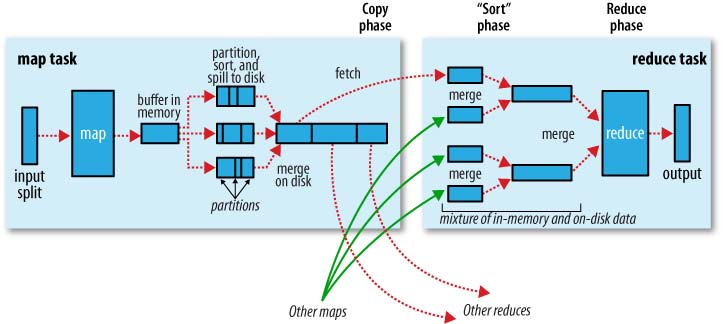
\includegraphics[scale=0.6]{images/shuffle_sort_mapred.png}
  \caption{\textit{shuffle} et \textit{sort} dans MapReduce. \\Source : O'Reilly | Hadoop: The Definitive Guide}
  \label{fig:shuffle-sort-mapred}
\end{figure}

\par Chaque \textit{map} possède un buffer circulaire dans lequel celui-ci écrit les données en sortie. Sa taille par défaut est de 100MB mais peut être modifiée à l'aide de la propriété \texttt{io.sort.mb}. Lorsque le contenu du buffer atteint un certain seuil (par défaut : 80\% paramétrable avec \texttt{io.sort.spill.percent}), un thread est lancé en fond chargé de transférer le contenu du buffer dans le disque du n\oe{}ud. Par abus de langage, ce thread peut être appelé : \textit{spill} (c'est le terme anglais désignant l'opération réalisée). Ainsi, les données en sortie du \textit{map} vont continuellement être écrites dans le buffer jusqu'à ce que le \textit{spill} soit lancé. Le cas de blocage de la fonction \textit{map} apparaît lorsque le buffer se remplit. Dans ce cas, la fonction \textit{map} attend que le thread \textit{spill} le vide pour continuer.

\par Cependant, avant d'écrire les données sur le disque, celles-ci sont partitionnées selon les \textit{maper} vers lesquelles elles seront envoyés par la suite. Chaque partition est ensuite triée ce qui permettra d'accélérer le \textit{reducer}. Remarquons que plusieurs threads \textit{spill} peuvent être créés. En effet, rien n'empêche d'atteindre le seuil après la création d'un thread en ce que l'opération \textit{map} peut être plus rapide que le thread. Ce raisonnement nous amène à considérer l'existence de plusieurs threads et nous comprenons qu'à chaque création d'un thread il devient de plus en plus difficile d'atteindre à nouveau le seuil.

\par Avant la fin de la fonction \textit{map}, l'ensemble des partitions est regroupé (\textit{merge}) en une seule et même partition triée par clé et prête à être envoyée à un \textit{reducer}. Les partitions en sortie des \textit{maper} sont ensuite acheminées vers les  \textit{reducers} par le biais du protocole HTTP.

\paragraph{La fonction \textit{reduce}} Cette fonction prend en entrée les sorties des différentes \textit{maps}. Ces dernières peuvent se terminer à des instants différents les unes des autres; instant pouvant varier en fonction du matériel utilisé et des données stockées. Ainsi, le les \textit{reducers} commencent à copier les données en \textit{streaming}. C'est la phase de copiage réalisée par plusieurs threads du \textit{reducer} qui vont recopier les données en parallèle. La valeur par défaut est cinq mais reste paramétrable.

\par Maintenant il est question de connaître les données en sortie des \textit{maps} que le \textit{reducer} doit copier. Pour ce faire, au fur et à mesure de l'exécution du job au sein des n\oe{}uds \textit{map} des signaux d'état (\textit{heartbeat}) sont envoyés aux noeuds maîtres qui sont le JobTracker (Hadoop 1.x) ou le ResourceManager (Hadoop 2.x). A leur tour ils renseignent aux \textit{reducers} l'emplacement des données à copier. Les données stockées dans les \textit{mapers} ne sont effacées qu'à la fin du job et ce afin de pallier à une quelconque panne.

\par Les données recueillies sont regroupées au fur et à mesure en partitions de taille définies. Lorsque la phase de copiage (\textit{copying phase}) est terminée et qu'un certain nombre de tailles définies ont été créés, la phase de trie (\textit{sort phase}) démarre.

\par L'invocation de la fonction \textit{reduce} pour chaque clé sur les données réorganisées et triées marque le début de la phase de réduction (\textit{reduce phase}). Le pré-tri réalisé dans les étapes précédentes prend tout son intérêt ici. En effet, l'ensemble des \texttt{valeurs} associées à une certaine \texttt{clé} se trouvent à la suite. La fonction \textit{reduce} est par conséquent optimisée en ce qu'elle s'épargne un tri pouvant s'exécuter sur des millions de paires. La sortie de cette phase est écrit  directement sur HDFS. L'utilisateur est ensuite en mesure de récupérer les données.


%\par La figure~\ref{fig:mapreduce-exp} donne l'aperçu global du patron MapReduce. Les données présentées en entrée sont splittées. Concrètement, les données splittées correspondent tout simplement aux blocs stockés dans les DataNodes des fichiers (cf \ref{sec:hdfs}). C'est sur ces données que va s'exécuter la fonction \textit{map} dans un premier lieu. La particularité c'est que c'est le code qui est envoyé sur les noeuds esclaves et non les données qui y sont déjà présentes. En terme d'I/O, les performances de calculs sont considérablement augmentées puisqu'on s'épargne le temps de transfert des données.
%
%\par Plusieurs fonctions \textit{map} peuvent s'exécuter simultanément. Ceci est possible du fait de l'architecture maître-esclave. La parallélisation des calculs augmente donc le temps de traitement.
%
%\subsection{Les I/O}
%\label{sec:mapreduce-io}
%
%\par Dans un algorithme MapReduce, les données présentes en entrée/sortie des tâches \textit{map} et \textit{reduce} sont toujours sous la forme \texttt{<key, value>} ou \texttt{<clé, valeur>}. Imposer cette structure unique et simple aux enregistrements contribue à l'efficacité d'Hadoop au niveau des I/O.
%
%\subsection{La fonction \textit{map}}
%
%\par Le programme le plus simple permettant de comprendre le patron MapReduce est le \texttt{wordcount}. Celui-ci permet de compter le nombre d'occurrences des mots d'un ou plusieurs fichiers. Afin d'illustrer la fonction nous prenons cet exemple. Le code source Java ainsi que les \texttt{input} et \texttt{output} sont joints à ce rapport.
%
%\paragraph{Le << parsage >> des données.} Un fichier texte en entrée de la fonction \textit{map} est traitée de façon très spécifique. En effet, la fonction \textit{map} prend en entrée une ligne du fichier. Le fichier ci-dessous
%
%\begin{quote}
%banane wiki mangue mac toto\\
%mac kiwi galaxy banane kiwi\\
%\end{quote}
%
%présenté en entrée de la fonction \textit{map} du \texttt{wordcount} produira le jeu de <clé, valeur> suivant :\\
%
%\centerline{
%\begin{tabular}{|c|c|}
%\hline  1ère phrase & 2ème phrase \\ 
%\hline banane, 1 & mac, 1\\wiki, 1 & kiwi, 1\\ mangue, 1 & galaxy, 1\\ mac, 1 & banane, 1\\ toto, 1 & kiwi, 1\\
%\hline 
%\end{tabular}} 
%
%\subsection{La fonction \textit{reduce}}

%%% Local Variables: 
%%% mode: latex
%%% TeX-master: "CompteRendu"
%%% End: 

% Configuration préalables à l'installation d'Hadoop
\section{Pré-requis de configuration Hadoop 1.2.1}

\subsection{Généralités}

\par Sortie le 1er août 2013, la version 1.2.1 de Hadoop est considérée stable. Ce document donne les étapes nécessaires à l'installation de ce framework Java. Installation et compréhension des concepts ne sont pas à porté de main. Ce guide ne prétend pas être exhaustif, le lecteur sera amené à chercher des informations par lui-même.

\par Pour de plus amples renseignements sur cette version, rendez-vous sur :\\
\emph{http://hadoop.apache.org/docs/r1.2.1/}

\subsection{Matériel utilisé}

\par L'installation effectuée dans le cadre de notre projet a été réalisée sur un MacBook Pro sous OSX 10.9.2 Mavericks datant de fin 2011 et doté d'un processeur 2,4 GHz Intel Core i5. Matériel et OS utilisés sont importants en ce qu'une compilation de Hadoop sera nécessaire dans certains cas.

\subsection{Création d'un nouvel utilisateur}

\par L'installation de Hadoop sur votre ordinateur est effectuée dans une première partie en mode \emph{Single Node}, autrement dit Hadoop ne déploiera ses calculs que sur votre machine, contrairement au mode \emph{Multi-Node Cluster} dans lequel plusieures machines sont agrégées dans le but d'augmenter la puissance de calcul.

\par Configurer Hadoop fait appel à l'écriture sur des fichiers susceptibles, en cas de mauvaise utilisation, d'altérer le bon fonctionnement de votre machine. Il est par conséquent conseillé de créer un nouvel utilisateur. De ce fait, \texttt{hduser} fait référence tout au long de ce document à l'utilisateur dédié à Hadoop. Celle-ci devra posséder les droits administrateur.

\subsection{Installation de Java}

\par Une fois le nouvel utilisateur Hadoop créé, ouvrez la session. Hadoop nécessite une version de Java supérieure à la version \texttt{1.5} afin d'assurer son bon fonctionnement. 

\par Pour connaître la version installée sur votre machine, ouvrez votre Terminal et tapez :

\begin{minted}[frame=single,mathescape]{bash}
ThiDiff:~ hduser$ java -version
\end{minted}

\par Ci-dessous vous pouvez constater que la version Java installée est la 1.7.

\begin{minted}[frame=single,mathescape]{bash}
java version "1.7.0_21"
Java(TM) SE Runtime Environment (build 1.7.0_21-b12)
Java HotSpot(TM) 64-Bit Server VM (build 23.21-b01, mixed mode)
\end{minted}

\par Dans le cas où une version de Java en-dessous de 1.5 est installée, rendez-vous sur \emph{http://www.java.com/fr} et suivez les instructions de téléchargement et d'installation.

\subsection{Configuration du SSH}

\par L'accès aux différents noeuds via Hadoop nécessite de configurer le SSH (\emph{Secure Shell}). Dans notre mode de fonctionnement, seule la configuration du \texttt{localhost} est nécessaire. La configuration du mode \emph{Multi-Node} est traitée dans la partie~\ref{sec:hadoop-2.2}.

\par Pour ce faire, vous devez générer une clé SSH pour votre session \texttt{hduser}. Sur votre Terminal, tapez :

\begin{minted}[frame=single,mathescape]{bash}
ThiDiff:~ hduser$ ssh-keygen -t rsa -P ""
Generating public/private rsa key pair.
Enter file in which to save the key (/Users/hduser/.ssh/id_rsa) :
Created directory /Users/hduser/.ssh .
Your identification has been saved in /Users/hduser/.ssh/id_rsa.pub.
80:37:49:f6:47:35:d1:86:85:00:39:d1:f0:8e:d3:8a hduser@ThiDiff.local
The key s randomart image is:
+--[ RSA 2048]----+
|      o +*oo+*.  |
|     + ooo. o.o  |
|    . = ..o  .   |
|     . o =       |
|        S o      |
|       . o       |
|      E .        |
|                 |
|                 |
+-----------------+
\end{minted}

\par Tapez sur la touche Entrée. La seconde ligne de commande ci-dessus génère la clé RSA avec un mot de passe vide. De façon général ceci n'est pas conseillé mais étant donné que nous ne travaillons qu'en local, cela ne pose aucun problème de sécurité.

\par Désormais nous devons autoriser l'accès SSH sur notre machine à l'aide de la clé RSA générée. Pour ce faire, vous devez autoriser cette clé en la plaçant dans le fichier \texttt{authorized\_keys} contenant la liste des clés autorisées. Pour cela :

\begin{minted}[frame=single,mathescape]{bash}
ThiDiff:~ hduser$ cat $HOME/.ssh/id_rsa.pub >>$HOME/.ssh/authorized_keys
\end{minted}

\par La connexion SSH sur votre machine est théoriquement possible. Pour rappel, votre machine est nomée \texttt{localhost}.

\begin{minted}[frame=single,mathescape]{bash}
ThiDiff:~ hduser$ ssh localhost
The authenticity of host 'localhost (127.0.0.1)' cannot be established.
RSA key fingerprint is 6c:8b:6f:43:42:ee:f3:27:ca:af:28:ea:51:08:a4:21.
Are you sure you want to continue connecting (yes/no)? yes
Warning: Permanently added 'localhost' (RSA) to the list of known hosts.
\end{minted}

\par Lors de votre première connexion, votre machine est enregistrée dans la liste des hôtes connus. Ainsi, à la prochaine connexion elle sera reconnue et la saisie du mot de passe de votre session n'est plus nécessaire. 

\par Pour vous déconnecter, rien de plus simple :

\begin{minted}[frame=single,mathescape]{bash}
ThiDiff:~ hduser$ logout
Connection to localhost closed.
\end{minted}

%%% Local Variables: 
%%% mode: latex
%%% TeX-master: "CompteRendu"
%%% End: 


% Installation d'Hadoop
\section{Hadoop 1.2.1}
\subsection{Préparation d'Hadoop}

\par Actuellement il est possible de trouver sur le serveur Apache toutes les versions de Hadoop. Cependant il est préférable de travailler avec des versions considérées comme stables. C'est notamment le cas pour les versions 1.2.x, 2.2.x et 2.3.x. Notre projet est basé sur la version 1.2.1.

\par Sur le lien ci-dessous, téléchargez le fichier hadoop-1.2.1.tar.gz  (61 Mb) :\\
\textit{http://apache.mirrors.multidist.eu/hadoop/common/hadoop-1.2.1/}

\par Une fois téléchargé, décompressez le fichier, renommez-le en hadoop et placez le dans /usr/local. Il est de plus très important de changer le propriétaire de ce fichier :

\begin{verbatim}
Ordinateur-ThiDiff:~ Hadoop$ cd /Users/Hadoop/Downloads
Ordinateur-ThiDiff:~ Hadoop$ mv hadoop-1.2.1 hadoop
Ordinateur-ThiDiff:~ Hadoop$ mv hadoop /usr/local
Ordinateur-ThiDiff:~ Hadoop$ sudo chown Hadoop hadoop
\end{verbatim}

\par Vérifiez que le nouveau propriétaire du fichier hadoop est bien votre session Hadoop :

\begin{verbatim}
Ordinateur-ThiDiff:~ Hadoop$ cd /usr/local
Ordinateur-ThiDiff:local Hadoop$ ls -lisa | grep hadoop
26284444  0 drwxr-xr-x@  29 Hadoop   admin    986  3 mai 14:12 hadoop
\end{verbatim}

\par Hadoop téléchargé, il faut désormais configurer quelques fichiers propres à Hadoop et qui font sa spécificité. Par conséquent, on ne parle par  d'installation mais plutôt de configuration car il s'agit tout au long de définir les bonnes propriétés.

\subsection{Débriefing du dossier hadoop}

\par Le dossier hadoop contient de nombreux sous-dossier qui ne sont pas tous aussi utiles les uns que les autres. En voici la liste :

\begin{verbatim}
CHANGES.txt		docs					ivy.xml
LICENSE.txt		hadoop-ant-1.2.1.jar			lib
NOTICE.txt		hadoop-client-1.2.1.jar			libexec
README.txt		hadoop-core-1.2.1.jar			logs
bin			hadoop-examples-1.2.1.jar		sbin
build.xml		hadoop-minicluster-1.2.1.jar		share
c++			hadoop-test-1.2.1.jar			src
conf
\end{verbatim}

\par Nous nous attardons que sur les dossiers bin et conf qui se sont montrés essentiels lors de notre étude d'Hadoop, laissant ainsi le lecteur s'intéresser de plus près aux autres fichiers.

\par A titre anecdotique, les fichiers hadoop-*.jar contiennent les librairies nécessaires à la compilation et à l'exécution des exemples contenus notamment dans le fichier hadoop-examples-1.2.1.jar (WordCount, etc...).

\par Ci-dessous quelques fichiers contenus dans le dossier bin que vous aurez à utiliser sans cesse par la suite afin de lancer Hadoop.

\begin{verbatim}
start-all.sh			stop-all.sh			
\end{verbatim}

\par Ces scripts shell vont permettent de lancer ou d'arrêter les différents démons d'Hadoop à savoir : le NameNode (NN), le DataNode, le SecondaryNameNode, le JobTracker et le TaskTracker. Pour de plus amples détails référez-vous à la partie détaillant chaque démon. Par conséquent, il sera possible de tout lancer simultanément ou de lancer au fur et à mesure chaque démon à l'aide des autres scripts.

\par Le dossier conf est le plus important de tous car il contient les fichiers permettant de configurer Hadoop. Quatre fichiers ont leur grande importance et qui seront détaillés par la suite :

\begin{verbatim}
hadoop-env.sh			mapred-site.xml
core-site.xml			hdfs-site.xml
\end{verbatim}

\subsection{Le fichier .bashrc}

\par Le fichier .bashrc fait parti des fichiers lus lorsque le shell est invoqué comme shell interactif sans fonction de connexion. Il est essentiel de définir quelques variables de l'environnement Hadoop dans ce dernier. Celui-ci se trouve dans \$HOME, si ce n'est pas le cas il suffit de le créér et devra contenir les informations ci-dessous.

\begin{verbatim}
# Hadoop environment variables
export JAVA_HOME=/Library/Java/JavaVirtualMachines/jdk1.7.0_21.jdk
		  /Contents/Home
export HADOOP_HOME=/usr/local/hadoop

# Add Hadoop bin/ dir to PATH Hadoop autocompletion commands
export PATH=$PATH:$HADOOP_HOME/bin
export PATH=$PATH:$HADOOP_HOME/sbin
export HADOOP_MAPRED_HOME=$HADOOP_HOME
export HADOOP_COMMON_HOME=$HADOOP_HOME
export HADOOP_HDFS_HOME=$HADOOP_HOME
\end{verbatim}

\par Hadoop a recours à Java, c'est pourquoi JAVA\_HOME est défini. Les autres variables définies permettent de définir les dossiers sur lesquels Hadoop devra être amené à travailler.

\subsection{Le fichier hadoop-env.sh}

\par Ce fichier contient les variables d'environnement nécessaires à Hadoop. Pour notre installation, seule la variable JAVA\_HOME doit être précisée. Pour l'obtenir, tapez la commande cat \$(/usr/libexec/java\_home). Votre fichier doit contenir :

\begin{verbatim}
# The java implementation to use.  Required.
export JAVA_HOME=/Library/Java/JavaVirtualMachines/jdk1.7.0_21.jdk
		  /Contents/Home
\end{verbatim}

\subsection{Les fichiers *-site.xml}

\par Les trois fichiers *-site.xml permettent de configurer le dossier où Hadoop stock les fichiers de données, les ports utilisés, le nombre de réplication des blocs, etc.

\subsubsection{core-site.xml}

\par Ce fichier XML contient les informations générales d'Hadoop. Entre autres, il définit le dossier dans lequel Hadoop stockera les données temporaires lors de l'exécution des tâches. Il définit aussi le nom et le port du système de fichiers qui a rendu célèbre Hadoop : HDFS (\textit{Hadoop Distributed File System}).

\begin{verbatim}
<configuration>

<property>
	<name>hadoop.tmp.dir</name>
	<value>/app/hadoop/tmp</value>
	<description>A base for other temporary directories.</description>
</property>

<property>
   <name>fs.default.name</name>
   <value>hdfs://localhost:54310</value>
 </property>

</configuration>
\end{verbatim}

\par /app/hadoop/tmp est le dossier contenant les données temporaires stockées par Hadoop aussi bien pour le système de fichier local que HDFS. Créez ce dossier et donnez-lui tous les droits d'accès :

\begin{verbatim}
Ordinateur-ThiDiff:~ Hadoop$ sudo mkdir -p /app/hadoop/tmp
Ordinateur-ThiDiff:~ Hadoop$ sudo chown Hadoop /app/hadoop/tmp
Ordinateur-ThiDiff:~ Hadoop$ sudo chmod 750 /app/hadoop/tmp
\end{verbatim}

\par Ne pas donner l'intégralité des droits à la session Hadoop produira une exception java.io.Exception lors du formatage du NameNode (confère partie suivante).

\subsubsection{mapred-site.xml}

\par Rappelons-le, Hadoop a deux principales composantes : HDFS et MapReduce. Ce fichier permet de configurer le deuxième point et plus particulièrement le JobTracker qui est le service d'Hadoop permettant de suivre les tâches. Pour cela on lui attribut un port sur lequel, à travers une interface web comme nous verrons plus loin, allons venir lire les informations concernant les jobs.

\begin{verbatim}
<configuration>

<property>
	<name>mapred.job.tracker</name>
    <value>localhost:54311</value>
</property>

</configuration>
\end{verbatim}

\subsubsection{hdfs-site.xml}

\par Ce dernier fichier définit les propriétés relatives au système de fichiers propre à Hadoop : HDFS. On y définit particulièrement le nombre de réplications des blocs. Nous ne nous attarderons pas d'avantage sur ce point à l'heure actuelle.

\begin{verbatim}
<configuration>

<property>
	<name>dfs.replication</name>
	<value>1</value>
</property>

</configuration>
\end{verbatim}

\par La configuration basique d'Hadoop en mode \textit{Single Node} ne nécessite que la modification des fichiers mentionnés précédemment. Pour le mode \textit{Multi Node} nous verrons que les fichiers /conf/masters et /conf/slaves auront leur importance.

\subsection{Formatage du NameNode}

\par La dernière étape restante avant de pouvoir lancer des jobs Hadoop est de formater le NameNode. Ce service Hadoop est la pièce maîtresse de HDFS en ce qu'il conserve l'arborescence de tous les fichiers HDFS au sein des DataNodes. Il contient par conséquent l'ensemble des métadonnées des fichiers HDFS.

\par Le formatage du NameNode permet d'effacer l'ensemble des données de HDFS. C'est équivalent à un RAZ. Cette étape n'est à réaliser qu'une seule fois lors de la mise en place de votre cluster Hadoop sous risque de perdre toutes les données HDFS présentes sur votre cluster.

\begin{verbatim}
ordinatrthidiff:~ Hadoop$ $HADOOP_HOME/bin/hadoop namenode -format
14/06/01 00:18:33 INFO namenode.NameNode: STARTUP_MSG: 
/************************************************************
STARTUP_MSG: Starting NameNode
STARTUP_MSG:   host = ordinatrthidiff/192.168.1.66
STARTUP_MSG:   args = [-format]
STARTUP_MSG:   version = 1.2.1
STARTUP_MSG:   build = https://svn.apache.org/repos/asf/hadoop/common/branches/branch-1.2 -r 1503152; compiled by 'mattf' on Mon Jul 22 15:23:09 PDT 2013
STARTUP_MSG:   java = 1.7.0_21
************************************************************/
14/06/01 00:18:35 INFO util.GSet: Computing capacity for map BlocksMap
14/06/01 00:18:35 INFO util.GSet: VM type       = 64-bit
14/06/01 00:18:35 INFO util.GSet: 2.0% max memory = 1013645312
14/06/01 00:18:35 INFO util.GSet: capacity      = 2^21 = 2097152 entries
14/06/01 00:18:35 INFO util.GSet: recommended=2097152, actual=2097152
2014-06-01 00:18:35.649 java[10479:1b03] Unable to load realm info from SCDynamicStore
14/06/01 00:18:36 INFO namenode.FSNamesystem: fsOwner=Hadoop
14/06/01 00:18:36 INFO namenode.FSNamesystem: supergroup=supergroup
14/06/01 00:18:36 INFO namenode.FSNamesystem: isPermissionEnabled=true
14/06/01 00:18:36 INFO namenode.FSNamesystem: dfs.block.invalidate.limit=100
14/06/01 00:18:36 INFO namenode.FSNamesystem: isAccessTokenEnabled=false accessKeyUpdateInterval=0 min(s), accessTokenLifetime=0 min(s)
14/06/01 00:18:36 INFO namenode.FSEditLog: dfs.namenode.edits.toleration.length = 0
14/06/01 00:18:36 INFO namenode.NameNode: Caching file names occuring more than 10 times 
14/06/01 00:18:38 INFO common.Storage: Image file /app/hadoop/tmp/dfs/name/current/fsimage of size 112 bytes saved in 0 seconds.
14/06/01 00:18:38 INFO namenode.FSEditLog: closing edit log: position=4, editlog=/app/hadoop/tmp/dfs/name/current/edits
14/06/01 00:18:38 INFO namenode.FSEditLog: close success: truncate to 4, editlog=/app/hadoop/tmp/dfs/name/current/edits
14/06/01 00:18:38 INFO common.Storage: Storage directory /app/hadoop/tmp/dfs/name has been successfully formatted.
14/06/01 00:18:38 INFO namenode.NameNode: SHUTDOWN_MSG: 
/************************************************************
SHUTDOWN_MSG: Shutting down NameNode at ordinatrthidiff/192.168.1.66
************************************************************/
\end{verbatim}

\par Hadoop est désormais configuré. L'étape suivante consiste à lancer les différents services Hadoop.

\subsection{Lancement des services Hadoop}

\par A chaque fois que vous souhaitez lancer les services Hadoop vous devrez suivre les étapes suivantes :

\begin{itemize}
\item se connecter via SSH au localhost;
\item forcer la lecture du fichier .bashrc à l'aide de la commande "source .bashrc";
\end{itemize}

\par Il suffit ensuite de lancer le script shell fournit dans le dossier Hadoop (/bin/start-all.sh) :

\begin{verbatim}
ordinatrthidiff:~ Hadoop$ start-all.sh
starting namenode, logging to /usr/local/hadoop/libexec/../logs/hadoop-Hadoop-namenode-ordinatrthidiff.out
localhost: starting datanode, logging to /usr/local/hadoop/libexec/../logs/hadoop-Hadoop-datanode-ordinatrthidiff.out
localhost: starting secondarynamenode, logging to /usr/local/hadoop/libexec/../logs/hadoop-Hadoop-secondarynamenode-ordinatrthidiff.out
starting jobtracker, logging to /usr/local/hadoop/libexec/../logs/hadoop-Hadoop-jobtracker-ordinatrthidiff.out
localhost: starting tasktracker, logging to /usr/local/hadoop/libexec/../logs/hadoop-Hadoop-tasktracker-ordinatrthidiff.out
\end{verbatim}

\par On voit sur la sortie que le NameNode, le DataNode, le SecondaryNameNode, le JobTracker et le TaskTracker se sont lancés. Cependant il est bon de vérifier leur état à l'aide de la commande jps (\textit{Java Virtual Machine Process Status Tool}).

\begin{verbatim}
ordinatrthidiff:~ Hadoop$ jps
10649 DataNode
10891 TaskTracker
10560 NameNode
10803 JobTracker
11087 Jps
10737 SecondaryNameNode
\end{verbatim}

\par Nous sommes désormais sûrs que les services Hadoop se sont lancés correctement. En effet, il se peut que NameNode ou le DataNode ne se lancent pas. Dans ce cas la solution la plus radicale et la plus efficace consiste à formater à nouveau le NameNode. Pour ce faire, vous devez arrêter les services et suivre la démarche détaillée précédemment.

\subsection{Arrêt des services Hadoop}

\par L'arrêt des services Hadoop s'effectue avec :

\begin{verbatim}
ordinatrthidiff:~ Hadoop$ stop-all.sh
stopping jobtracker
localhost: stopping tasktracker
stopping namenode
localhost: stopping datanode
localhost: stopping secondarynamenode
\end{verbatim}

%%% Local Variables: 
%%% mode: latex
%%% TeX-master: "CompteRendu"
%%% End: 


% Exemples de traitements "Big Data"
\section{Applications}

\par La configuration Hadoop fournit des exemples plus ou moins complexes dans le but de se familiariser avec cet environnement. A titre d'exemple, dans l'archive hadoop-examples-1.2.1.jar nous retrouvons l'algorithme MapReduce permettant d'estimer la valeur de $\pi$. Afin de mieux comprendre le patron d'architecture MapReduce traitons un cas concret de multiplication de matrices.

\subsection{Multiplication de matrices}
\label{sec:matmult}

\par Dans le cadre de l'électif STAGVOD (\textit{Stockage et accès à de gros volumes de données}) nous avons été une première fois initiés à Hadoop. L'enseignant s'est particulièrement intéressé à l'algorithme MapReduce permettant de multiplier deux matrices qui est un très bon exemple de compréhension du fonctionnement des méthodes \textit{map} et \textit{reduce}. Vous trouverez en annexe le fichier Mm.java contenant l'implémentation des fonctions.

\subsubsection{La fonction \textit{main}}

\par \textit{map} prend comme entrée un fichier contenant les matrices. Compte tenu de l'implémentation de l'algorithme, il est indispensable que fichier en entrée soit de la forme suivante :

\indent A : [0 1 2 3 4] [5 6 7 8 9]\\
\indent B : [0 1 2] [3 4 5] [6 7 8] [9 10 11] [12 13 14]

\par Ci-dessous vous trouverez la fonction main :

\begin{minted}[frame=single,linenos,mathescape]{java}
public static void main(String[] args) throws Exception {

	if (args.length < 2) {
		System.exit(0);
	}
	
	Configuration conf = new Configuration();
	// A is an L-rows, M-cols matrix
	// B is an M-rows, N-cols matrix.
	conf.set("L", "2");   
	conf.set("M", "5");
	conf.set("N", "3");

	Job job = new Job(conf, "MatrixMultiplication");
	
	[...]
}
\end{minted}

\par Tout d'abord il est essentiel d'initialiser la configuration où le contexte viendra puiser ses données en précisant la taille des matrices. Par conséquent, à chaque changement de matrices, il faudra à nouveau définir la taille des matrices. Le job est ensuite créé sur la base de cette configuration.

\par Le reste de la fonction définit les chemins vers les fichiers .class des fonctions \textit{map} et \textit{reduce}, les formats de la paire (clé, valeur) ainsi que le format des fichiers en entrée et sortie (ici texte).
  
\subsubsection{La fonction \textit{map}}

\par Le fichier texte en entrée sera d'abord traité par cette fonction. \textit{map} le lit ligne par ligne le fichier et pour chaque ligne s'exécute une fois. Ce fichier est dans un premier temps splitté au caractère ":" et la lettre A est stockée dans matStruc[0] et les coefficients de cette matrice dans matStrut[1] (valable pour B aussi). A partir de là, un nouveau tableau, matLines, contenant les lignes est créé de telle sorte que \smallskip:\\
\smallskip
Pour la matrice A\\
matLines[0]=[0 1 2 3 4\\
\smallskip
matLines[1]=[5 6 7 8 9\\
Pour la matrice B\\
matLines[0]=[0 1 2\\
matLines[1]=[3 4 5\\
matLines[2]=[6 7 8\\
matLines[3]=[9 10 11\\
matLines[4]=[12 13 14\\

\par Selon que ce soit la matrice A ou B, un traitement différent est opéré. En effet, dans le produit de matrices C=A*B, les coefficients de A et B mis en jeu dans le calcul du coefficient (i,j) de C ne sont pas les mêmes. D'où cette distinction.

\par Que ce soit pour A ou B, les tableaux à double entrée créés au début sont remplis avec la valeur des coefficients des matrices correspondantes. (A[0][0]=0, A[0][1]=1, etc...). Le reste du code se charge de créer les paires (clé, valeur). La clé correspond au coefficient de la matrice C. La valeur correspond à un des coefficients mis en jeu dans le produit matriciel.

\par Pour exemple on a :
\begin{verbatim}
(C_0_0, (A,0,A[0][0]))  (C_1_0, (A,0,A[1][0]))
(C_0_0, (A,1,A[0][1]))	(C_0_0, (A,1,A[1][1]))
(C_0_0, (A,2,A[0][2]))	(C_0_0, (A,2,A[1][2]))
(C_0_0, (A,3,A[0][3]))	(C_0_0, (A,3,A[1][3]))
(C_0_0, (A,4,A[0][4]))	(C_0_0, (A,4,A[1][4]))
\end{verbatim}

\par Le fichier mm\_mapreduce\_explication.txt contient l'ensemble des paires (clé, valeur) des matrices A et B en sortie de la fonction \textit{map}.

\subsubsection{La fonction \textit{reduce}}

\par "mapper" les matrices revient à parser les coefficients des matrices en leur faisant correspondre le coefficient de C dans lequel il est impliqué. A ce stade, l'ensemble des paires (clé, valeur) nécessaires à la multiplication puis addition pour le calcul des coefficients de C ont été obtenues.

\par Le rôle de la fonction \textit{reduce} est d'isoler la bonne ligne de A et la bonne colonne de B auxquelles ont assigne la bonne clé. Elle va ainsi récupérer par clé les lots de deux vecteurs (celui associé à A et celui associé à B) correspondant à un élément scalaire de la matrice finale, puis multiplier deux à deux leurs éléments et les sommer.

\par Par exemple pour C00 on a :

\begin{verbatim}
    (C_0_0, (A,0,A[0][0]))   x   (C_0_0, (B,0,B[0][0]))\\
 +  (C_0_0, (A,1,A[0][1]))   x   (C_0_0, (B,1,B[1][0]))\\
 +  (C_0_0, (A,2,A[0][2]))   x   (C_0_0, (B,2,B[2][0]))\\
 +  (C_0_0, (A,3,A[0][3]))   x   (C_0_0, (B,3,B[3][0]))\\
 +  (C_0_0, (A,4,A[0][4]))   x   (C_0_0, (B,4,B[4][0]))\\
 =	 C_0_0 final
\end{verbatim}

\par Hadoop n'est pas du tout adapté au multiplication de matrices. Ceci est un exemple dans le but unique de comprendre l'algorithme MapReduce. Le fichier de sortie obtenu se trouve en annexe sous le nom output\_matmult.txt.

%%% Local Variables: 
%%% mode: latex
%%% TeX-master: "CompteRendu"truct.
%%% End: 


% Conclusion
\section{Conclusion}

\par Ce projet fut beaucoup plus long que prévu. En effet, nous avons sous-estimé les difficultés à installer Hadoop. Il aura été nécessaire de réunir des connaissances diverses, liées à l'environnement d'installation. Par conséquent, des approfondissements de la syntaxe du bash ainsi que du fonctionnement de SSH auront précédé l'installation définitive de Hadoop sur le cluster Skynet. Le wordcount s'est donc déroulé avec succès sur 17 noeuds (\texttt{sh00} à \texttt{sh16}).
\par Désormais, nous pouvons nous intéresser à l'aspect ``performances'' de Hadoop, et également à la possibilité d'utiliser des programmes rédigés dans un autre langage que Java, grâce à la fonctionnalité \emph{Streaming} de Hadoop.

%%% Local Variables: 
%%% mode: latex
%%% TeX-master: "CompteRendu"
%%% End: 


\end{document}
